\chapter{THỰC HIỆN ĐỀ TÀI}
\section{Yêu cầu hệ thống}
\paragraph{}
Hệ thống thiết bị phải được lắp đặt và lập trình cho các công việc sau:
\begin{itemize}
    \item Khi cấp nguồn thực hiện truyền dòng chữ "Họ và tên sinh viên là: " lên màn hình console của máy tính qua giao tiếp uart.
    \item Khi người dùng gõ các ký tự lên màn hình console, dữ liệu được gửi sang thiết bị và hiển thị trên màn hình LCD1602 cũng như gửi lại ký tự lên màn hình console để hiển thị cho người gõ.
    \item Nếu ký tự người dùng gõ không phải ký tự chữ cái, chữ số, dấu cách hoặc ký tự xuống dòng, bỏ qua ký tự.
    \item Nếu người dùng nhấn "Enter", thực hiện gửi chuỗi "Đã nhập: " và chuỗi người dùng nhập vào lên màn hinh máy tính, hiển thị trên màn hình LCD1602 dòng chữ "TEN SINH VIEN LA" và dòng 2 là chuỗi người dùng nhập.
    \item Nếu người dùng nhấn Enter sau lần nhấn Enter trước đó, thiết bị gửi chuỗi xóa màn hình console và gửi dòng "Họ và tên sinh viên là: " lên màn hình console của máy tính. Khi người dùng nhập ký tự đầu tiên, thực hiện xóa màn hình LCD1602 và thực hiện in ký tự đó và các ký tự tiếp theo.
\end{itemize}

\paragraph{}
Một số yêu cầu phi chức năng khác:
\begin{itemize}
    \item Hệ thống cần đáp ứng nhanh, xử lý nhanh tránh trường hợp người dùng cảm nhận được độ trễ khi nhập.
    \item Khi người dùng nhập ký tự nhanh (từ 20ms), không được làm mất ký tự.
    \item Nhận đúng ký tự người dùng nhập vào và hiển thị đúng ký tự đó lên màn hình console cũng như màn hình LCD1602.
    \item Số ký tự tối đa được nhập dưới 100 ký tự, nếu vượt quá khoảng hiển thị của màn hình LCD1602, thực hiện thuật toán cuộn trang để hiển thị các ký tự.
\end{itemize}
\section{Lựa chọn và lắp đặt phần cứng}
\subsection{Sơ đồ phần cứng}
Đối với phần cứng, kết nối giữa module \acrshort{i2c} và \acrlong{mcu} được thực hiện như trong bảng \ref{tab:lcd-wiring} để sử dụng ngoại vi I2C1.

\begin{table}[H]
    \centering
    \caption{Chân kết nối màn hình LCD}
    \begin{tabular}{|c|c|}
        \hline
        Chân vi điều khiển & Chân module \acrshort{i2c} \\
        \hline
        PB8 (SDA) & SDA \\
        \hline
        PB9 (CLK) & CLK \\
        \hline
        GND & GND \\
        \hline
    \end{tabular}
    \label{tab:lcd-wiring}
\end{table}

\paragraph{}
Thiết bị chuyển USB sang UART được sử dụng là module CMSIS-DAP, tích hợp sẵn khả năng nạp chương trình qua chuẩn SWD và chuyển đổi USB sang UART. Sau khi kết hối các thiết bị, ta có sơ đồ như trong hình \ref{fig:dev-block}.

\begin{figure}[H]
    \centering
    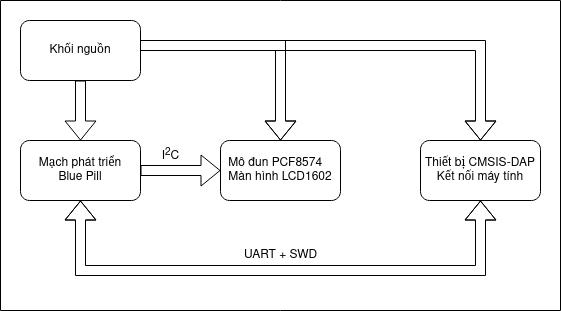
\includegraphics[width=0.8\textwidth]{images/arm-co-ban-device-block-diagram.drawio.png}
    \caption{Sơ đồ các thiết bị của hệ thống}
    \label{fig:dev-block}
\end{figure}
\subsection{Phần cứng thực tế sau khi ghép nối}

\section{Các thành phần phần mềm}

\subsection{Lựa chọn công cụ phát triển}
Rust là một ngôn ngữ lập trình mới có triển vọng trong nhiều lĩnh vực trong đó có lĩnh vực lập trình cho thiết bị nhúng. Vì vậy, nhóm quyết định phát triển hệ thống bằng ngôn ngữ này. Ứng dụng cho mảng nhúng, một số điểm mạnh của ngôn ngữ Rust bao gồm:
\begin{itemize}
    \item Hệ thống kiểu dữ liệu mạnh mẽ giúp tránh các lỗi liên quan đến bộ nhớ cũng như về luồng. Giúp chương trình chạy an toàn và dễ dàng đúng với mong muốn đặt ra hơn. Ví dụ như trong quản lý ngắt, luồng ngắt và luồng chính sẽ không thể gây ra sai xót về dữ liệu khi sử dụng Rust.
    \item Dữ liệu được quản lý an toàn mà không yêu cầu trình dọn rác. Điều này đặc biệt quan trọng do các thiết bị nhúng thường có cấu hình không cao.
    \item Các thư viện mã nguồn mở đa dạng, thân thiện với người dùng hơn nhờ hệ thống kiểu dữ liệu đa dạng, có thể tích hợp các phương thức giống lập trình hướng đối tượng trong khi vẫn đảm bảo các chức năng cấp thấp cần thiết cho lập trình nhúng.
    \item Trình biên dịch mạnh mẽ, giúp phát hiện lỗi ngay từ khi lúc biên dịch. Khi chương trình biên dịch thành công là chương trình có thể hoạt động được. Lỗi logic không thể được phát hiện nên cần được kiểm tra kỹ.
\end{itemize}

\paragraph{}
Môi trường phát triển dựa trên trình soạn thảo Neovim có tích hợp công cụ rust-analyzer cho việc lập trình Rust. Công cụ gỡ lỗi sử dụng probe-run giúp quá trình phát triển dễ dàng hơn.
\begin{figure}[H]
    \centering
    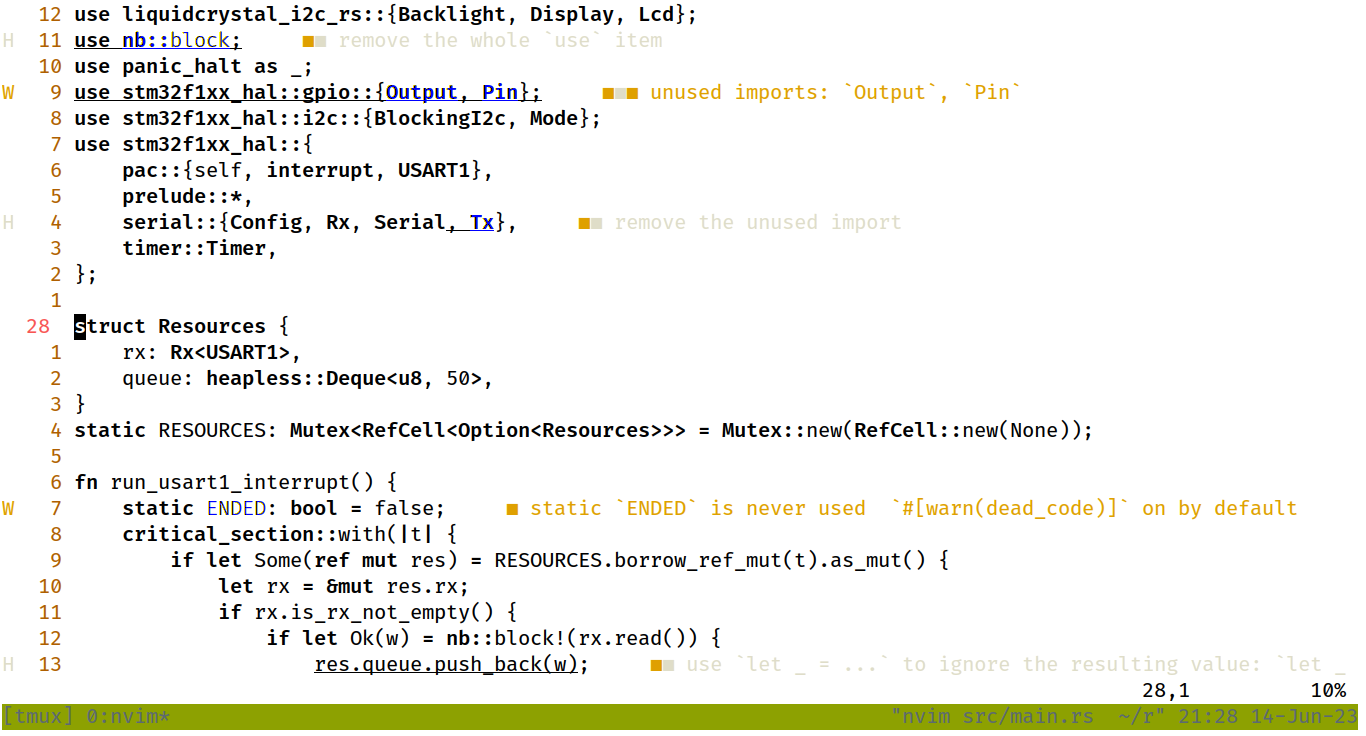
\includegraphics[width=0.8\textwidth]{images/Screenshot from 2023-06-14 21-28-38.png}
    \caption{Môi trường lập trình trên Neovim và rust-analyzer}
    \label{fig:neovim-environment}
\end{figure}


\subsection{Lựa chọn các thư viện}
\paragraph{}
Các thư viện cần thiết khi lập trình cho thiết bị nhúng bao gồm thư viện hỗ trợ phần cứng HAL và các thư viện đặc biệt giúp thao tác với các thiết bị ngoại vi được gắn thêm. Ngoài ra, các phần mềm 
\subsection{Triển khai phần mềm}

\section{Đánh giá}

\subsection{Kết quả đạt được}
Hệ thống đã đảm bảo đầy đủ theo các chức năng như đề ra trong đề tài. Hệ thống đã được xây dựng với các thiết bị phần cứng và phần mềm đúng như yêu cầu môn học đưa ra.
Thời gian hiển thị tương đối chính xác theo giờ tiêu chuẩn.

\subsection{Hạn chế của hệ thống}
Hệ thống đã đạt được mong muốn đề ra nhưng cũng không tránh khỏi những sai sót. Do hệ thống được phát triển ở mức thực nghiệm nên thiết kế sản phẩm có sơ sài về mặt kết nối các phần cứng. Đôi khi kết nối chập chờn dẫn đến sai sót trong hiển thị.
